\documentclass[12pt, a4paper,oneside, nocenter]{thesis}

%setting font to Arial
\usepackage[T1]{fontenc}
\usepackage[scaled]{uarial}
\renewcommand*\familydefault{\sfdefault} 

\usepackage{graphicx}%package for imges
\usepackage{float}

\usepackage[hyphens]{url}
\def\UrlBreaks{\do\/\do-}
\usepackage[hyphenbreaks]{breakurl}
\urlstyle{same}

\usepackage{xcolor}
\usepackage{etoolbox}
\usepackage{setspace}
\usepackage{wallpaper}
\usepackage{lipsum}
%\usepackage[none]{hyphenat}
%remove hyphenation
\tolerance=1
\emergencystretch=\maxdimen
\hyphenpenalty=10000
\hbadness=10000

\usepackage[document]{ragged2e}
\usepackage[font=small,labelfont=normal,figurename=Figure,labelsep=period]{caption} % Required for specifying captions to tables and figures
\captionsetup{justification=raggedright,singlelinecheck=false}

\usepackage[margin=1in,top=0.5in,includehead=true]{geometry}

\usepackage{cleveref}%setting figure referencing
\crefname{figure}{(Figure}{(Figure}
\creflabelformat{figure}{#2\textup{#1}#3)}
%%%%%%%%%%%%%%%%%%%%%%

\usepackage{titlesec}
\assignpagestyle{\chapter}{fancy}

% \ignore command for inline comments
\newcommand{\ignore}[2]{\hspace{0in}#2}

%Setting new line margins
\renewcommand{\baselinestretch}{1.5}

\usepackage{tocloft}%changing table of contents to dots
\renewcommand{\cftsecleader}{\cftdotfill{\cftdotsep}} % for sections
\renewcommand{\cftpartleader}{\cftdotfill{\cftdotsep}} % for parts
\renewcommand{\cftchapleader}{\cftdotfill{\cftdotsep}} % for chapters
\renewcommand\cftchapfont{\normalfont\fontsize{12}{12}\selectfont} % chapter font to 12\12
\renewcommand\cftchappagefont{\normalfont\fontsize{12}{12}\selectfont} %chapter page number font to 12\12

%headheight resetting error
\setlength{\headheight}{15pt}% ...at least 51.60004pt
%disabling identation for paragraphs
\setlength{\parindent}{0cm}
%increasing space before chapter
\setlength{\cftbeforechapskip}{2.5pt}

%style for chapters
\titleformat{\chapter}
[hang]
{\normalfont\fontsize{12}{12}\selectfont\bfseries}
{\thechapter}
{1em}{}

\titlespacing*{\chapter}{0pt}{-0.2cm}{0.3cm}
\titleformat*{\section}{\normalfont\fontsize{12}{12}\selectfont\bfseries}
\titleformat*{\subsection}{\normalfont\fontsize{12}{12}\selectfont\bfseries}
\titleformat*{\subsubsection}{\normalfont\fontsize{12}{12}\selectfont\bfseries}
\setlength{\parskip}{1em}

\usepackage{fancyhdr}%fancy headers/footers

\fancyhf{} % sets both header and footer to nothing
\fancyhead[C]{\thepage}

\fancypagestyle{plain}{%
\fancyhf{} % clear all header and footer fields
\fancyhead[C]{\thepage} %RO=right odd, RE=right even
\renewcommand{\headrulewidth}{0pt}
\renewcommand{\footrulewidth}{0pt}
}

\setcounter{section}{1}%start table of contents at 1

%-----------------------------------References------------------------------%
\usepackage[nottoc,notlot,notlof]{tocbibind}
\usepackage[comma]{natbib}
\bibliographystyle{dcu}

%move left
\setlength{\bibhang}{0pt}

\renewcommand\harvardurl[1]{\RaggedRight\textbf{URL:}
\url{#1}}

\renewcommand{\bibname}{REFERENCES}
%-------------------------------------------------------------------------------%


% used in title page
\author{Aleksandar Ivanov}
\title{Educational AR/VR Systems for military projects}

\AtBeginDocument{% setting contents name to uppercase
  \let\mtcontentsname\contentsname
  \renewcommand\contentsname{\MakeUppercase\mtcontentsname}
}

\newcommand\blankpage{% used for adding an empty page
    \null
    \thispagestyle{empty}%
    \addtocounter{page}{-1}%
    \newpage}

\pagestyle{plain}
%%%%%%%%%%%%%%%%%%
%%%%%%%%%%%%%%%%%%
%%%%%%%%%%%%%%%%%%
%%%%%%%%%%%%%%%%%%
%%%%%%%%%%%%%%%%%% BEGINNING OF DOCUMENT
%%%%%%%%%%%%%%%%%%
%%%%%%%%%%%%%%%%%%
%%%%%%%%%%%%%%%%%%
\begin{document}

\pagenumbering{gobble}%removing page counter
% Set the right side of the footer to be the page number\fancyhead[R]{\thepage}

\makeatletter
\begin{titlepage}
	\begin{center}
	\ThisLRCornerWallPaper{1}{background.png}
		\vspace*{2cm}
		{\fontsize{16}{16}{\selectfont\@author}}\par
		\vspace{1cm}
		
		{ \setstretch{2.0}
			\fontsize{24}{24}{\selectfont\MakeUppercase{\@title}}
			
		}
		
		\vspace{1.5cm}
		{\setstretch{1.2}
			\fontsize{16}{16}\selectfont Bachelor's thesis \\ Information Technology
			
		}
        	
		\vspace{1.5cm}
        
		\fontsize{16}{16}\selectfont\the\year
        
		\vfill
		
\includegraphics{xamklogo}
		\vspace{0.8cm}
	\end{center}
\end{titlepage}
\makeatother

\blankpage

\newpage%TOC page
{\setstretch{1.2}
\tableofcontents
}

\newpage%first page with content

\newgeometry{top=1.25cm,left=4.0cm,right=2cm,bottom=1.25cm, head=14.5pt, includehead,includefoot,
  heightrounded,headsep=1cm}
\pagenumbering{arabic}%starting page counter


%make title bold from outside so TOC stays the same
\chapter{\MakeUppercase{Introduction}}
Developments and improvements in computing technology have allowed for vastly improved immersion when consuming digital media. The most notable examples of such technologies are Augmented reality and Virtual reality. The immersion these technologies offer can be used to create educational systems that have more benefits than traditional digital educational systems. \par
In this thesis project I will be comparing the difference between AR(Augmented reality) and VR(Virtual reality) in the context of educational software. Different implementations and physical devices will be compared and analyzed. A device and a technology will be chosen to prototype an educational application for Observis Oy related to the company's Situational Awareness System(SAS).\par The SAS product has a steep learning curve which raises the need for a more efficient educational tool. The goal of the project is to pick the most suitable technologies and implement such a tool. Advantages and disadvantages of AR/VR need to be considered over more traditional digital educational tools.
\\
\chapter{\MakeUppercase{Augmenter Reality and Virtual Reality}}
Augmented reality and Virtual reality are technologies that offer a different view and experience to the physical world. They leverage similar kinds of technology and both aim to provide an enhanced and enriched experience to the user. Both technologies are a part of the general area of mixed reality \Cref{fig:reality-virtuality}. However they have different goals and are essentially different in terms of user experience.

\begin{figure}[H]
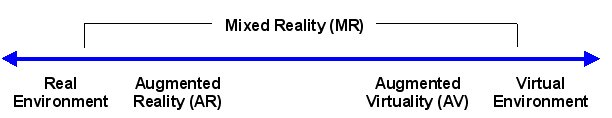
\includegraphics[width=\textwidth]{Virtuality_Continuum_2}
\caption{Reality-Virtuality Continuum (Paul Milgram et al. 2007)}
\label{fig:reality-virtuality}
\end{figure}

\section{Augmented Reality}%ref http://kjcomps.6te.net/upload/paper1%20.pdf
Augmented Reality can be described as the technology that bridges reality with virtual environments. Real life objects are transformed or replaced with virtual equivalents. Information can be added or removed to the real environment. Key aspects of AR(Augmented Reality) are the ability to run in real time, be interactive, three dimensional and combine real with virtual information. AR is most commonly used with the sense of sight, but it can potentially be used with other senses such as hearing, touch, smell, taste, temperature etc. Augmented Reality can be considered as the next step in graphical user interfaces(GUI) evolution\citep{prototyping-ar}. Its current state is comparable to command line interfaces and 2d interfaces in the 1980's and 1990's. It is a vision of future computing and a field that is under research.\par
Augmented Reality has higher technological requirements compared to VR which has lead to the slower maturity of AR. AR enabling technologies have been developed throughout the history of which the Optical see-through has become the most popular(Microsoft HoloLens, Google Glass, Intel's Vaunt). Optical see-through is achieved by using opaque displays on which virtual overlays can be rendered. The resolution of the real world is left intact as it passes through the screen. Benefits of this approach include power fail safety, which allows users to still see the real world even during a power outage, cheaper production costs of the used displays, no parallax effect that irritates the user's eyes. Disadvantages are the reduced visibility and brightness through the opaque lenses, limitation of the field-of-view, requirement of additional tracking sensors such as cameras, gyroscopes and accelerometers. Due to the lack of maturity of other AR enabling technologies only Optical see-through techniques will be considered throughout this work\citep{vrjournal}.
\subsection{AR for training and education}%ref https://files.eric.ed.gov/fulltext/ED510220.pdf
Augmented Reality provides new paths to conveying information. Learning experiences are more contextual by connecting and embedding information with the real world in real time. These approaches are already being utilised by Boeing. 
Mechanics in the company use AR goggles that aid repairs with embedded textual instructions, 
illustrate different steps of the repair and help users identify the required tools for a repair. 
Consequently training resources are reduced and transfer of information between workers is greatly 
improved\citep{horizon-report}.\par
Learning through doing is another approach in which AR shines. Mistakes and errors made during the learning
experience have no real consequences. This provides for more authentic learning experiences which cannot be
achieved in any other way\citep{augmented-reality}.
\subsection{AR Challenges}
% As most developing technologies AR has many challenges that need to be overcome or improved. The requirements of the AR framework
% are directly related to those challenges.
An AR framework has basic requirements to accomplish a combination of the real and virtual world.
The four main requirements are sensing, tracking, interaction and display\Cref{fig:ar-framework}. Sensing refers to
capturing environment events and recognising markers or other objects of interest. Tracking handles updating the
viewing direction and position of the user relative to the real world. Tracking is an important component
of AR as even a slight tracking error can cause misalignment between the virtual and real objects\citep{ar-design}. 
Registration refers to how the digital information is being delivered to the user. The registration can be achieved
through different methods for different senses: videos, audio, haptic feedback, scent, etc.
\begin{figure}[H]
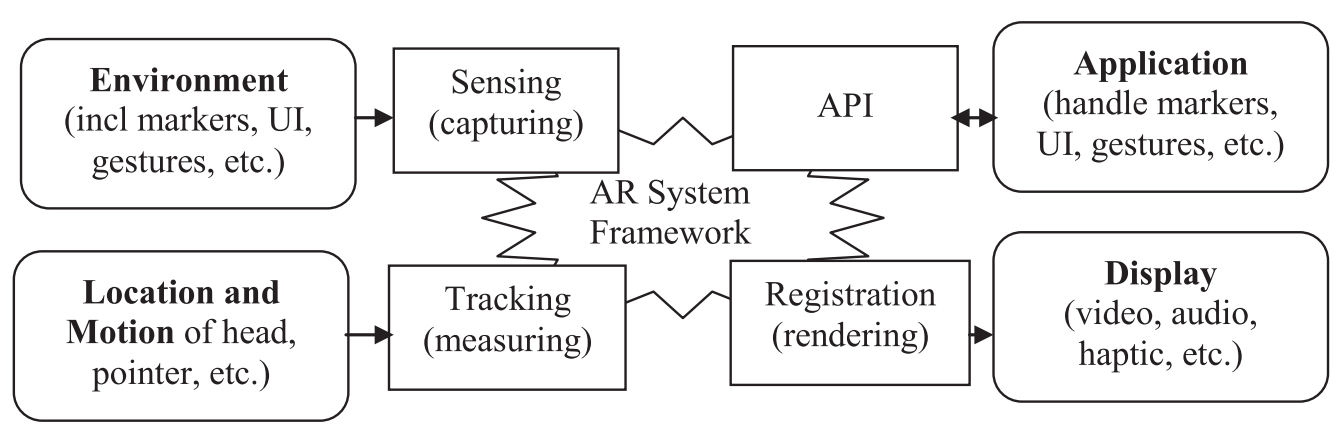
\includegraphics[width=\textwidth]{ar-framework}
\caption{Augmented Reality framework\citep{vrjournal}}
\label{fig:ar-framework}
\end{figure}
As most developing technologies AR has many challenges that need to be overcome before it can be widely adopted.
The challenges of AR arise from the framework requirements and they can be separated in five groups\Cref{fig:ar-challenges}.
\begin{figure}[H]
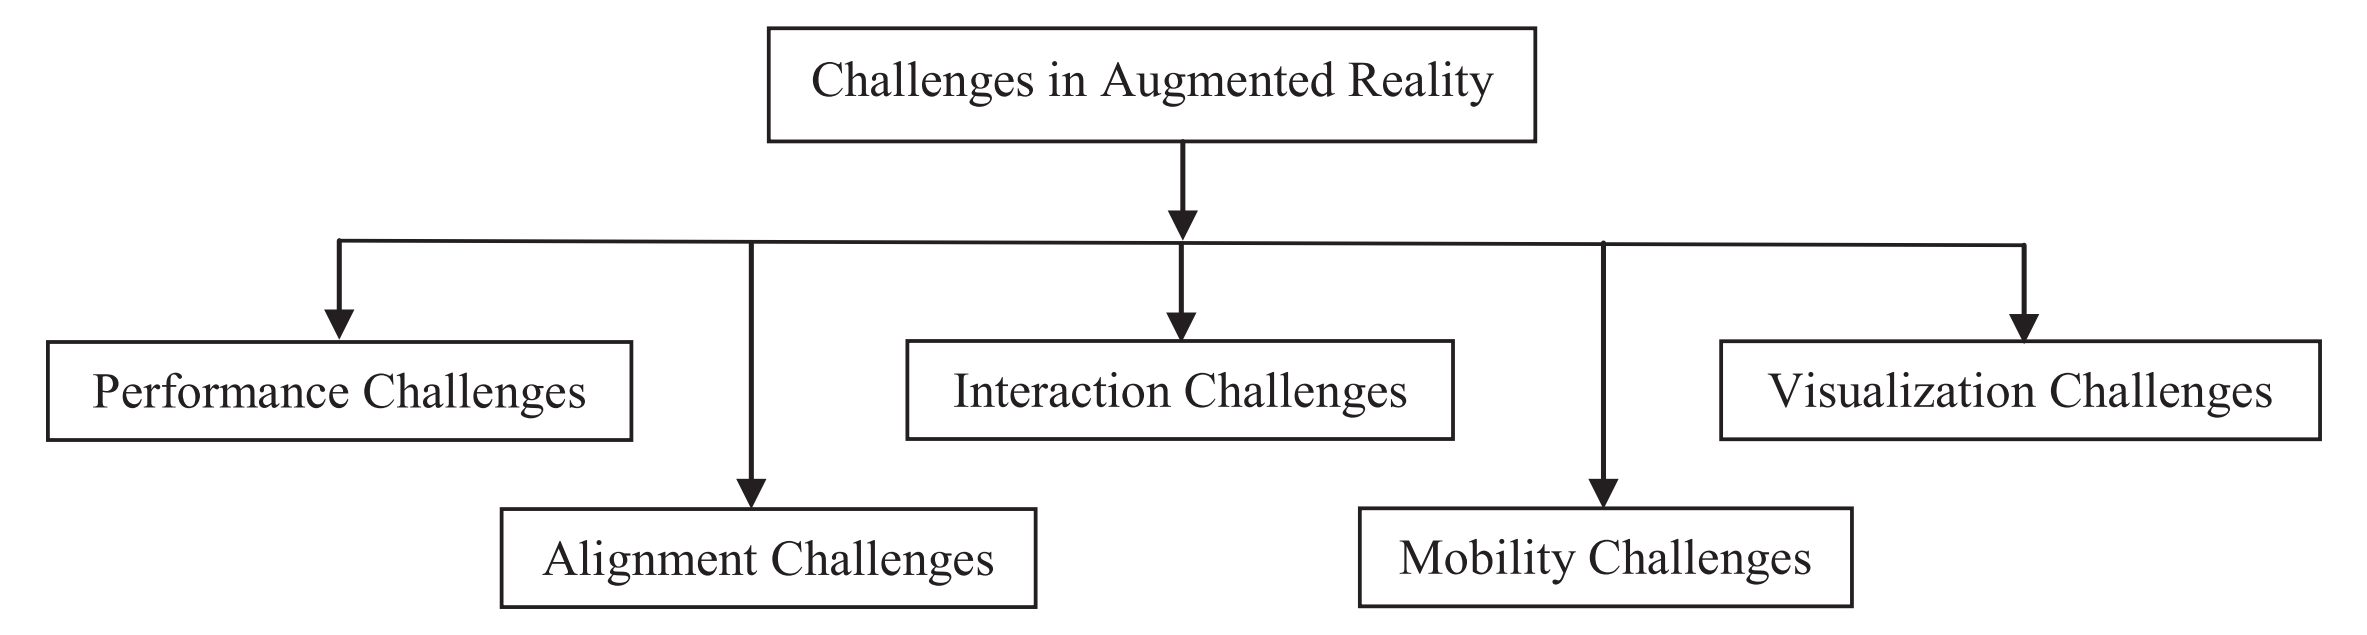
\includegraphics[width=\textwidth]{ar-challenges}
\caption{Augmented Reality challenges\citep{Acta-Graphica}}
\label{fig:ar-challenges}
\end{figure}
Performance challenges arise from the need of real time processing. AR tasks such as marker detection
and virtual object rendering are computationally intensive and this slows down performance.
Alignment challenges come from the complexity of tracking the users movement and registration of real
life objects. Any errors in those methods can cause misalignment between the rendered objects and
real view.\par
Interaction challenges are concerned with the interaction between users and virtual or real objects.
User interfaces need to be intuitive and unobstructive for the best experience. Mobility challenges refer
to the need of portability for AR systems.
\\
\section{Virtual Reality}
Virtual Reality in the broadest sense is the method or technology of substituting a physical environment with a virtually perceived environment.
This is typically achieved by using an HMD with integrated motion tracking and a built-in or external rendering unit.
The requirements of VR are same to those of AR with the exclusion of environment sensing\Cref{fig:ar-framework}. The virtual environment
is entirely digitally constructed, thus eliminating the need for sensing as all environmental events are native to the system.
\par
Interaction with the environment isn't necessary for a VR experience, but it increases the possibilities and usability of a VR system.
Different approaches to user interaction offer various degrees of immersion and limitations. Motion tracked controllers, hand motion tracking gloves, pointer centered to the viewport, headset location tracking in 3D space and sekeletal motion tracking are common approaches.
\subsection{VR Challenges}
VR challenges can be categorized in the same way as AR challenges\Cref{fig:ar-challenges}.
Performance is a very important factor in keeping the VR experience immersive for a prolonged period of time.
High resolution picture rendering at a high freamerate in real-time is taxing even for the highest end of current GPUs. 
Lower framerate or lower resolution picture can cause dizziness, eye tiredeness and overall dissatisfaction. Alignment challenges arise from the difficulty of tracking in real-time.
Users' view, location or controllers can become misaligned with the virtual environment, breaking the immersion and interactability.
Interaction challenges come from the current hardware limitations on interacting. Tactile feedback, hand interaction and free movement in the 3D space are all possible individually, but combining them at the same time is not yet achievable.
\par
Mobility challenges arise from the need of portability for VR platforms. Common solutions
rely on tethering to a machine that handles the rendering and power supply. However portable VR backpacks and headsets are starting to emerge\citep{hp-vrbackpack}.
Visualization can be difficult due to the complexity of the physical world. Keeping proportions, lighting, textures, view depth, field of vision and other visiual perception aspects can be challenging.
 



\par

\subsection{VR for education and training}
\section{Hybrid technologies}
\par
\chapter{\MakeUppercase{Project use case}}
\section{Comparing VR and AR in the project context}
\section{Researching mixed reality implementation}
\section{Risks and challenges to the mixed reality approach}
\section{Traditional approaches to training systems}
\par
\chapter{\MakeUppercase{Project implementation}}
\section{Defining the application specifications and requirements}
\section{Implementing basic scene with objects}
\section{Tracking and interacting with the virtual environment}
\section{Creating a context for training}

\par
\chapter{\MakeUppercase{Analyzing the mixed reality training application}}

\section{Future possibilities for development and improvement}


\newpage

\nocite{*}
\bibliography{references}

\end{document}
